%--------------------Chapter 4------------------------
\chapter{Knowledge Base Design: Ontology and Facts}

\hspace{0.3in} In Section 4.1, we give a brief introduction to ontologies and how light-weight RDFS ontologies are used to structure the facts in our eTourPlan KB. The descriptions of eTourPlan's FOAF-like profiles for the main tourist entities incorporating Bhutan tourist information used in eTourPlan are described in section 4.2. 

\section{Ontology Design}
\hspace{0.3in} Ontologies represent the real world in a systematically structured way. By consistently defining deep terms for the same real-world entities, ontologies provide a `reference model' for their domains, a strong set of terms which can be used to simplify communications between domain experts and therefore increase comprehension and knowledge sharing.

\hspace{0.3in} We represent the concepts (or `classes') of the tourism subdomains in RDF Schema (RDFS) light-weight ontologies, adapted from the Harmonise ontology, discussed earlier (Section 2.3). These ontologies are used to structure the FOAF-like profiles of the Bhutan tourism subdomains represented in POSL. 

\hspace{0.3in}RDFS provides modeling primitives for organizing (Web) objects into hierarchies. It is viewed as a basic language for writing light-weight ontologies that are subClassOf taxonomy. In RDFS, objects sharing similar characteristics can be typed with classes. Examples of eTourism classes are events, attractions, accommodations, etc.  Individuals belonging to a class are often referred to as instances of that class. For example, the ``2008\_Film\_Festival" can be an instance of the events class.

\hspace{0.3in}Classes can be grouped into hierarchies through the subClassOf relationship: a class C is a subclass of a class D if every instance of C is also an instance of D. For example, every instance of a cultural festival is an event instance since cultural festival is a subclass of the event class. Our ontology is adapted from the Harmonise ontology for the following reasons: 1) Harmonise is a mature and standard ontology used by many renowned tourism organizations, 2) It supports interoperability among many agents and applications in the tourism domain, and 3) It is expressed in RDFS, whose SubclassOf hierarchies are supported by our rule engine OO jDREW.

\section{Ontology and FOAF-like Profile Descriptions of eTourPlan}

We now look at each of the tourism subdomains considered in our eTourPlan prototype and their corresponding RDFS light-weight ontologies. The accommodation, attraction, and event subclasses are represented using RDFS subClassOf properties adapted from Harmonise ontology definitions. The administrative subdivision of a country such as Bhutan is implemented with partonomy rules, which are discussed later (Chapter 5). 
 
\hspace{0.3in} These ontologies are designed using Protege, which is an ontology-development tool used in such a way that it can provide the type definitions. The ontology is kept light-weight because currently OO jDREW supports only the subClassOf property. We also implemented certain RDFS domain and range restrictions of properties by using ``slots" in 
OO RuleML\footnote{\href{www.ruleml.org/ indoo/indoo.html}{\url{www.ruleml.org/ indoo/indoo.html}}}. Slotted facts and rules are represented in POSL where a typed slot becomes slot name -$>$ slot filler:filler type, where ``-$>$" is used for associating a slot name to a slot filler and ``:" is used for appending a filler type to a slot filler. This representation is used to describe profiles for each of the tourist entities. The classes (RDFS light-weight ontologies) provide the type definitions for each of the subdomains, and the instances of tourist entities for these classes are described with FOAF-like profile descriptions. The knowledge about any of the tourist entities can then queried by using the typed rule system OO jDREW.

\subsection{Province Profile}

\hspace{0.3in}Every tourist entity can be located in some administrative part of a country. Since provinces are the official top-level governmental administrative division of various countries, %into areas, 
we have designed FOAF-like profiles for provinces. Each of the province profiles includes information such as the URL, capital city, geographic details such as elevation and area. In addition, it also provides tourist information such as number of attractions, number of events and number of accommodations found in the province. The vocabularies that are borrowed from the Harmonise naming conventions are prefixed with an `hs', while those with `et' prefixes are the user-defined vocabulary for the eTourPlan KB. Namespaces are represented as prefixes before a `.' symbol\footnote{This is because the symbol `:', commonly used to express namespaces, as in many other languages is reserved in POSL as a type infix for separating terms from their order-sorted types.} for the purpose of implementation. It also has an ``hs.relatedTo" slot, used to provide the next adjoining province to visit. This FOAF-like relation among the province profiles forms a touristic route across the country. This aspect of connecting the 10 selected provinces of Bhutan, with respect to their neighbouring relations is shown in Figure 4.1. The FOAF relation among these related provinces is symmetric.

\begin{figure}
\begin{center}
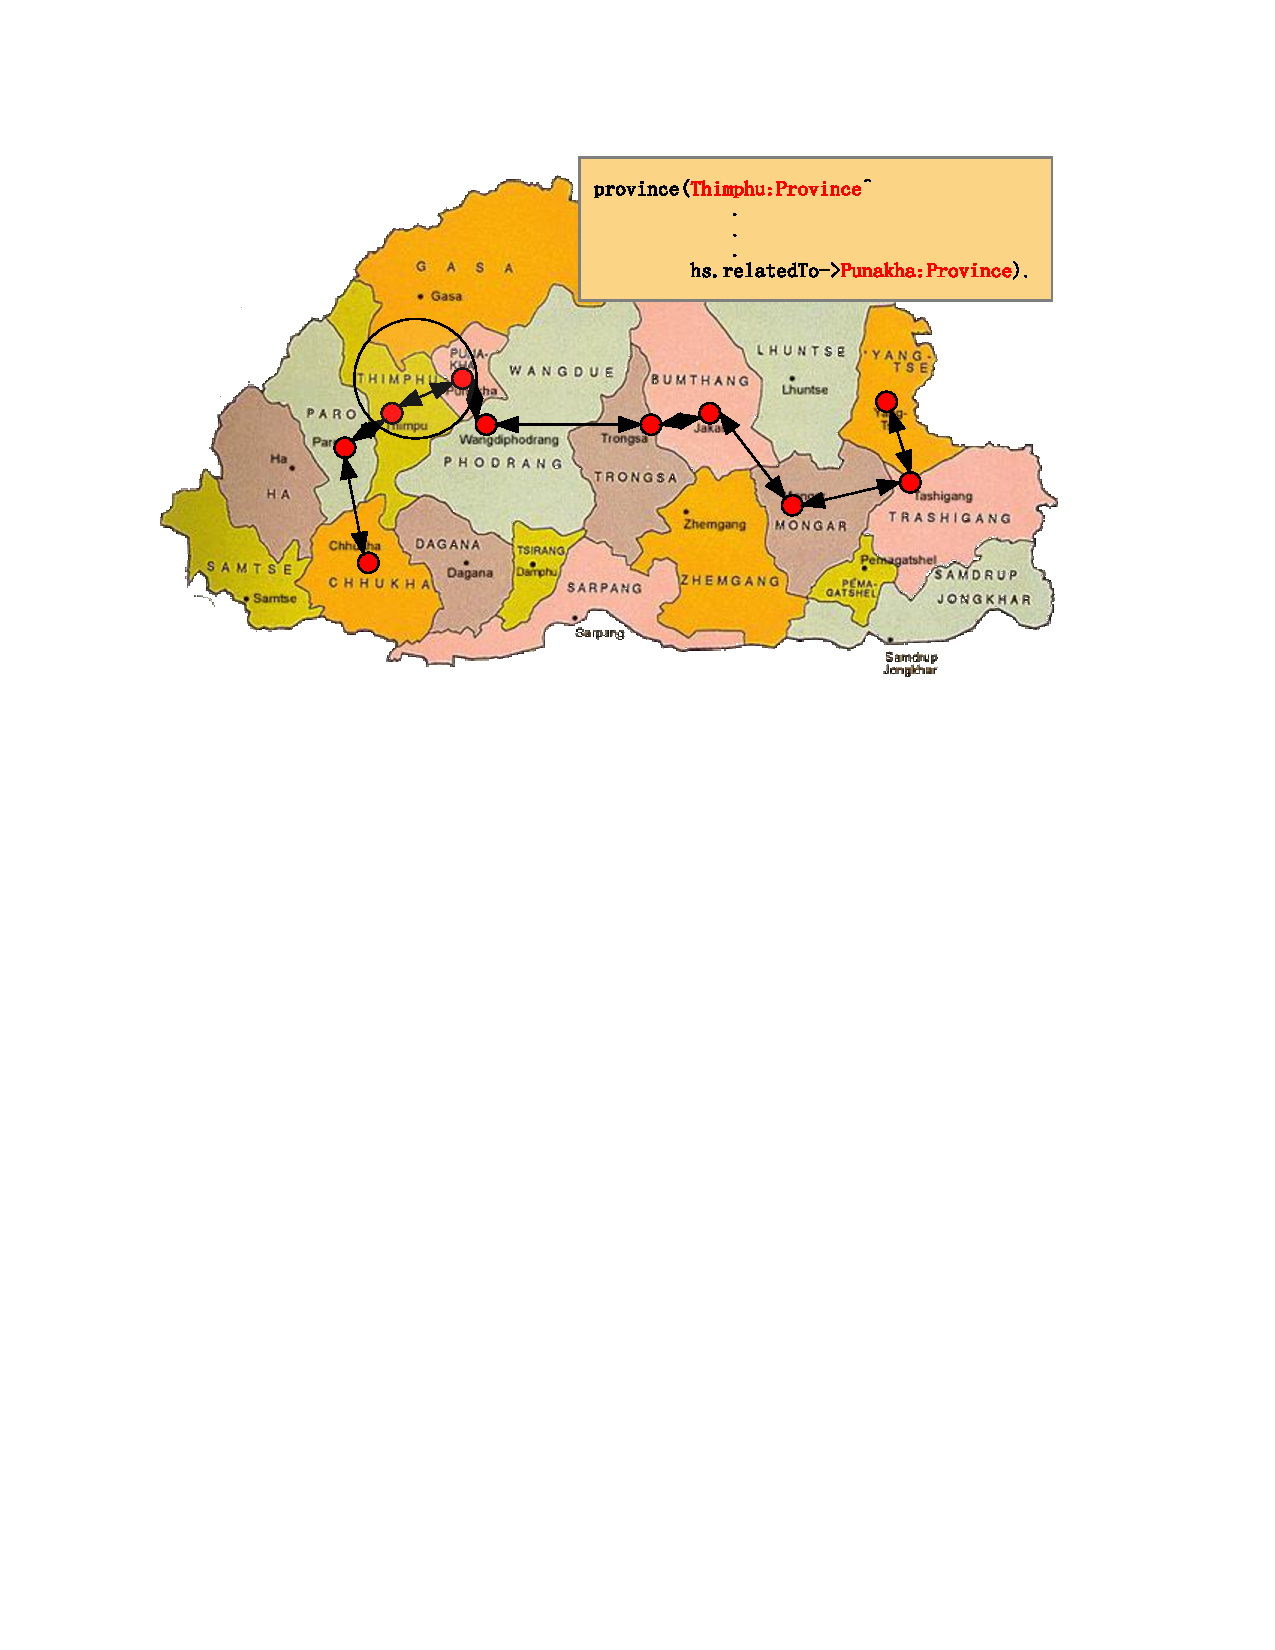
\includegraphics[width=13cm, height=7cm]{Provinces}
\caption {The relation between provinces in the KB}
\label{fig:Fig4.1}
\end{center}
\end{figure} 


\hspace{0.3in} We use the name of the province as the object identifier of its profile, and in POSL is represented before all the regular slots of our object-centric, slotted profile facts. The type of the object is attached to the object name with a colon infix (`:'). A hat symbol `$^{\wedge}$' is used to seperate the identifier from the rest of the slots (properties) in the profile. 
\\

\textbf{Profile of Thimphu Province}

\begin{small}
\singlespacing
\begin{verbatim} 
province(Thimphu:Province^
                 hs.url->"http://www.thimphu.gov.bt";
                 et.capital->Thimphu_City:City;
                 et.area->"1,819 sq.km";
                 et.elevation-> "1,300 to 7300 meters";
                 et.numBlocks->10:Integer;
                 et.numAttractions->3:Integer;
                 et.numEvents->2:Integer;
                 et.numAccommodations->0:Integer;
                 hs.languagesSpoken->"Dzongkha";
                 hs.description->"Thimphu is the capital of Bhutan";
                 hs.relatedTo->Punakha:Province).
\end{verbatim}
\end{small}

\hspace{0.3in}We want to note that these profile descriptions in POSL syntax are interconvertible to OO RuleML, and they can be tested in either of the syntax in the reasoning engine, OO jDREW. The detailed information about these province profiles (cf. Appendix B) can be extracted through queries in the OO jDREW TD reasoning engine. Such rules and queries are discussed later in chapters 5 and 6.

\subsection{Events Class}

\hspace{0.3in}The Events subdomain provides a model of a real-world event, characterized in terms of locations, timescale, theme, and other properties. Events are of two main types, periodic events and single occurrence events. An example of periodic event is `Sunday\_flea\_Market', which occurs once a week periodically, or an annual festival that occurs once a year on a particular date, whereas a single occurrence event occurs only once, like the ``Beijing\_2008\_Sum- mer\_Olympics". However, for the purpose of this thesis, we have considered both kinds of events under one category. The subclassOf hierarchy of the events subdomain is implemented by a light-weight ontology and the domain and range restrictions of other properties are represented in the FOAF-like fact instances of events in POSL format. The events class has nine subclasses, each of which is further subclassified into smaller classes as shown in Figure 4.2. This diagram was produced by Protege. An excerpt from the RDFS taxonomy describing a portion of the subClassOf hierarchy for the events class is shown below:

\singlespacing
Events

\hspace{10mm}Festival

\hspace{20mm}Annual\_festival

\hspace{20mm}Dance\_festival

\hspace{20mm}Film\_festival

\hspace{20mm}Gastronomic\_festival

\hspace{20mm}International\_festival

\hspace{20mm}Music\_festival

\hspace{20mm}National\_festival

\hspace{20mm}Seasonal\_festival

\hspace{20mm}Traditional\_festival\\

\begin{figure}
%\begin{center}
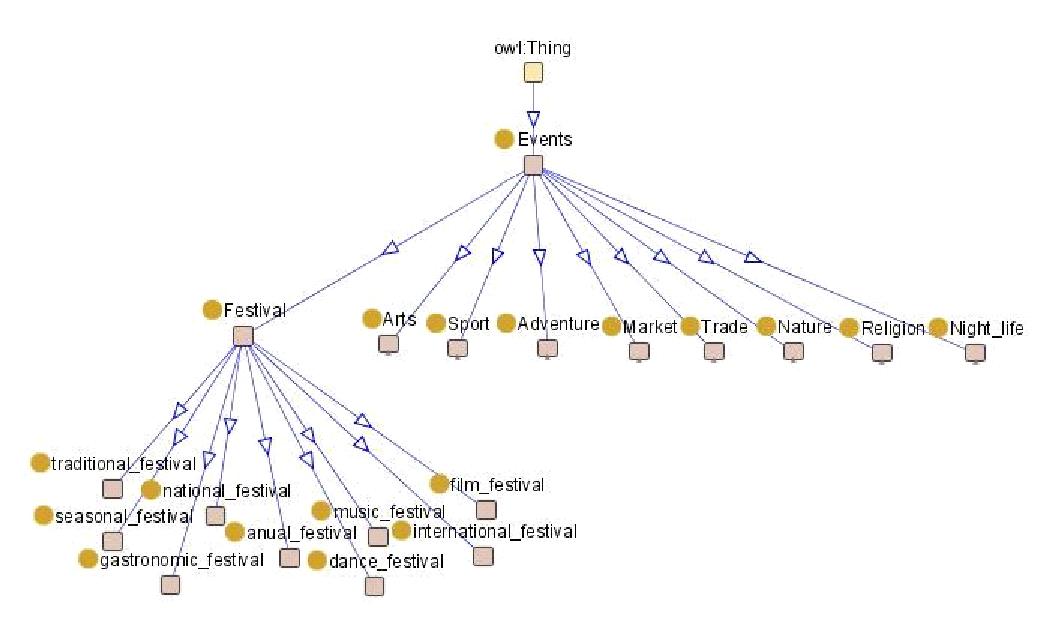
\includegraphics[width=15cm, height=9.5cm]{events}
\caption {Events class (full version in Appendix E)}
\label{fig:Fig4.2}
%\end{center}
\end{figure}


\doublespacing
\hspace{0.3in}The other subclasses of Events are Adventure, Arts, Market, Nature, Nightlife, Religion, Sport and Trade. The complete RDFS type hierarchy is shown in Appendix E. Each instance of the above classification for the Events subdomain is represented as FOAF-like profiles (cf. Appendix B). A FOAF-like profile of an instance of the Events class of type Annual\_festival is shown below:
\\
\\

\textbf{Profile of Thimphu\_Tshechu}

\begin{small}
\singlespacing
\begin{verbatim} 
event(Thimphu_Tshechu:Annual_festival^
                      hs.url->" ";
                      hs.startDate->date[2008:Real,10:Real,09:Real];
                      hs.endDate->date[2008:Real,10:Real,11:Real];
                      et.theme->Cultural_Religious_Heritage;
                      hs.location->Tashichoe_Dzong:Fortress;
                      et.province->Thimphu:Province;
                      hs.description->"It is a popular festival in Thimphu";
                      hs.relatedTo->Thimphu_Drupchen:Annual_festival).  
\end{verbatim}
\end{small}

\hspace{0.3in}The above slotted fact describes an event in Bhutan, ``Thimphu\_Tshechu" under the type Annual\_festival, along with other slots describing the event details. The ``hs.relatedTo" slot relates this event profile to the next upcoming event,  that is closest to this periodic event schedule. 


\subsection{Attractions Class}

\hspace{0.3in}This section presents the RDFS ontology of attractions. The Attraction subdomain considers attractions that are open to the public at a fixed location and are generally accessible throughout the year. An example of such an attraction could be a museum, a waterfall, or a park. The light-weight ontology for the attraction subdomain is shown in Figure 4.3. An excerpt from the RDFS taxonomy describing a portion of the subClassOf hierarchy for the attraction subdomain is shown below:

\singlespacing
Attractions

\hspace{10mm}Buildings

\hspace{20mm}Historical\_buildings

\hspace{30mm}Museum

\hspace{40mm}Local\_museum

\hspace{40mm}National\_museum

\hspace{40mm}Regional\_museum

\hspace{40mm}Private\_museum


\doublespacing

\begin{figure}
\begin{center}
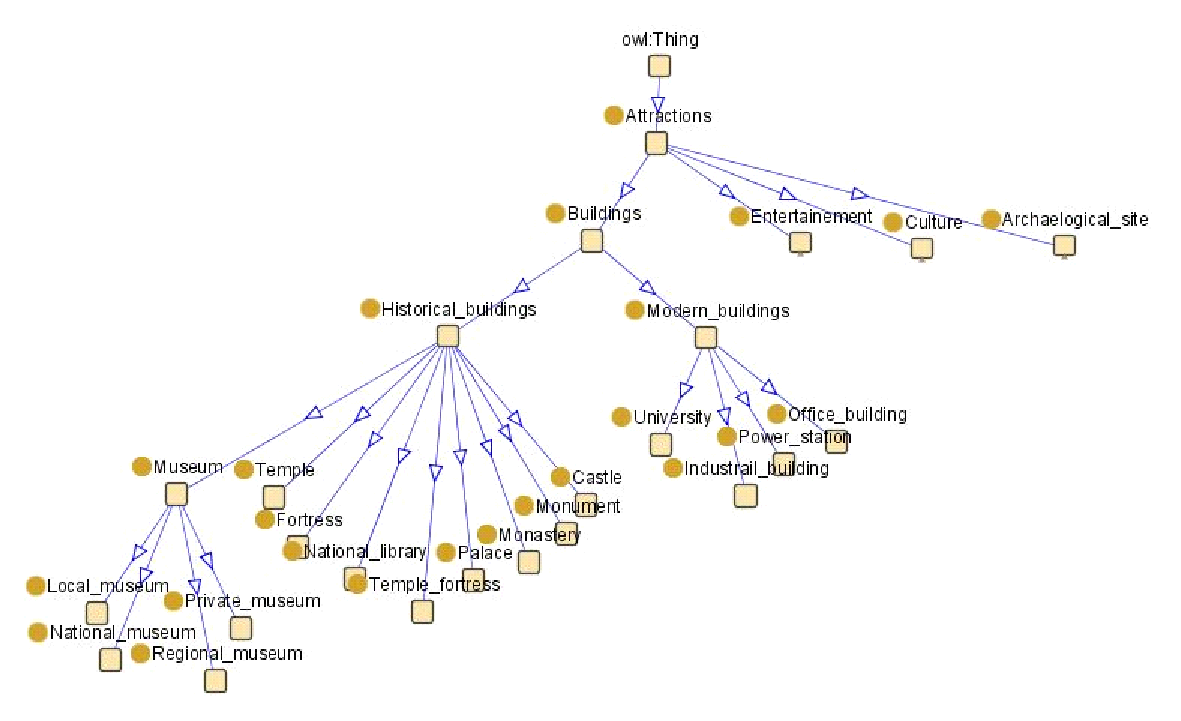
\includegraphics[width=15cm, height=9cm]{Attractions}
\caption {Attractions class (full version in Appendix E)}
\label{fig:Fig4.3}
\end{center}
\end{figure}


A FOAF-like profile for an instance of the Attractions class is shown below:
\\
\\

\textbf{Profile of Ta\_Dzong}

\begin{small}
\singlespacing
\begin{verbatim}
 attraction(Ta_Dzong:National_museum^
                     hs.url->"www.nationalmuseum.gov.bt/";
                     et.subblock->Goepay:Village;
                     et.province->Paro:Province;
                     et.theme->Cultural_Religious_Heritage;
                     et.open->Open[DaysOfWeek[Tue, Wed, Thu, Fri, Sat, Sun],
                                   Period[10:Real, 16:Real]];
                     et.capitalDistance->0.5:Real;
                     hs.description->"It is the biggest and the oldest museum
                                      in Bhutan";
                     hs.contact->" ";
                     hs.schedule->"12 months";
                     hs.relatedTo->Tashichoe_Dzong:Fortress).   
\end{verbatim}
\end{small}

\hspace{0.3in}The above slotted fact describes an attraction site, ``Ta\_Dzong", under the class National\_museum as its type, along with other slots describing the attraction. The ``hs.relatedTo" slot name in attraction profiles plays a very important role in connecting all the popular neighbouring attractions in the country. This property of our KB is later used to recommend and plan attraction-based travels, as discussed later (in Chapter 5).

\hspace{0.3in}An attraction has much in common with an accommodation and has many similar properties because both are static (i.e., they do not move from their place) and both are accessible most of the time. Both could have a price attribute but in this thesis, we have described price only for accommodations.

\subsection{Accommodations Class}
 
\hspace{0.3in} The accommodation class is subclassified into five main categories as shown in Figure 4.4. Our classification is a subclass of the Harmonise accommodation type definition. We have considered five related types in this thesis. A FOAF-like profile of an accommodation is shown below:
\\
\\
\\
\textbf{Profile of Wangdicholing\_Lodge}

\begin{small}
\singlespacing
\begin{verbatim} 
accommodation(Wangdicholing_Lodge:Lodge^
                            hs.url->"http://www.wangdicholing.bt/";
                            et.rating->3:Real;
                            et.minPrice->800:Real;
                            et.subblock->Chamkhar:Town;
                            et.province->Bumthang:Province;
                            hs.telecoms->Telecoms[
                                           et.landline->9753631452;
                                           et.cell->97517682948];
                            hs.contact->"manager@wangdicholing.bt";
                            hs.relatedTo->Yangphel_Guest_house:Guest_house).      
\end{verbatim}
\end{small}

\begin{figure}
\begin{center}
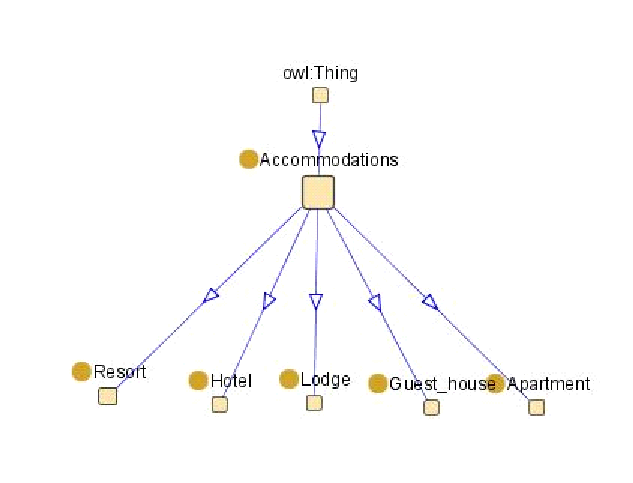
\includegraphics[width=11cm, height=5.1cm]{AccommodationClass}
\caption {Accommodations class}
\label{fig:Fig4.4}
\end{center}
\end{figure}

\hspace{0.3in}The above slotted fact describes an accommodation, ``Wangdicholing\_Lodge" under the class `Lodge'as its type, along with slots describing the accommodation such as the star rating, URL, minimum price, and a related accommodation. The ``hs.relatedTo" slot in the accommodation subdomain is used to link a profile to an accommodation of similar (ideally equal or nearly equal) rating within minimum distance in the same province.

\hspace{0.3in}We will now proceed to how the well-structured knowledge in our KB is used for implementing rules that operate on the aforementioned facts.







  
    
   


 
 




 

  
